%% The following is a directive for TeXShop to indicate the main file
%%!TEX root = diss.tex

\chapter{Luminescence from Organic Molecules}
\label{ch:opv}

Prior to the work done in this thesis, \ac{STML} from a single organic molecule has not yet been detected on our system. The system was designed by T. Roussy, and the plasmonic emission had been detected \citep{roussy2016coupling}. To optimize and ensure the viability of the experimental setup, \ac{STML} was performed on prototypical organic semiconducting molecules \ac{PTCDA} \citep{Rzeznicka2011, Kimura2019} and \ac{ZnPc} \citep{Zhang2016, Doppagne2017, Zhang2017, Imada2016, Doppagne2018, Miwa2019}, both of which have had successful reports of \ac{STML} experiments. Through the \ac{SPM} of individual molecules, we can explore the influence of the local environment on the optoelectronic properties of the organic semiconductor. Fluorination of phthalocyanine molecules has previously been used to tune the electronic and optical energies of the molecule in bulk \citep{schwarze2016band, warren2019controlling}. Further experiments were carried out on \ch{F8ZnPc} to explore the effects of fluorination on the structural, electronic and optical properties of ZnPc. 

During \ac{STML} experiments, the tip was parked on top of the molecule with a certain bias, and setpoint current. The shutter to the spectrometer was then opened for a certain exposure time ($t_x$).

\section{Plasmon emission from substrates}

Plasmon emission from the bare metallic surface can vary in energy and intensity depending on the geometry of the tip. Aside from attaining a sharp metallic tip for \ac{STM} and \ac{STS}, the tip needs to be poked and pulsed until it produces a strong plasmonic response in the energy region of interest. Representative spectra of the plasmon on Ag(111) and Au(111) with a Ag tip is presented in \autoref{fig:opv:metal-plasmon}. The same Ag tip was used to acquire both spectra, allowing for comparison. Due to the shift in tip-sample junction on Au(111), a result of the thinner substrate, the plasmon emission intensity was decreased by about an order of magnitude when compared to the Ag(111) substrate. The red-shift in photon energy was caused by the inherent dielectric response of the gold substrate \citep{olmon2012optical, yang2015optical}. 

% The shift in photon energy was because of the dielectric function of the two materials: gold with a minimal imaginary dielectric function at \SI{1.8}{eV} or \SI{680}{nm} \citep{olmon2012optical}, and silver at \SI{3.2}{eV} or \SI{390}{nm} \cite{yang2015optical}.

\begin{figure} [h]
    \centering
    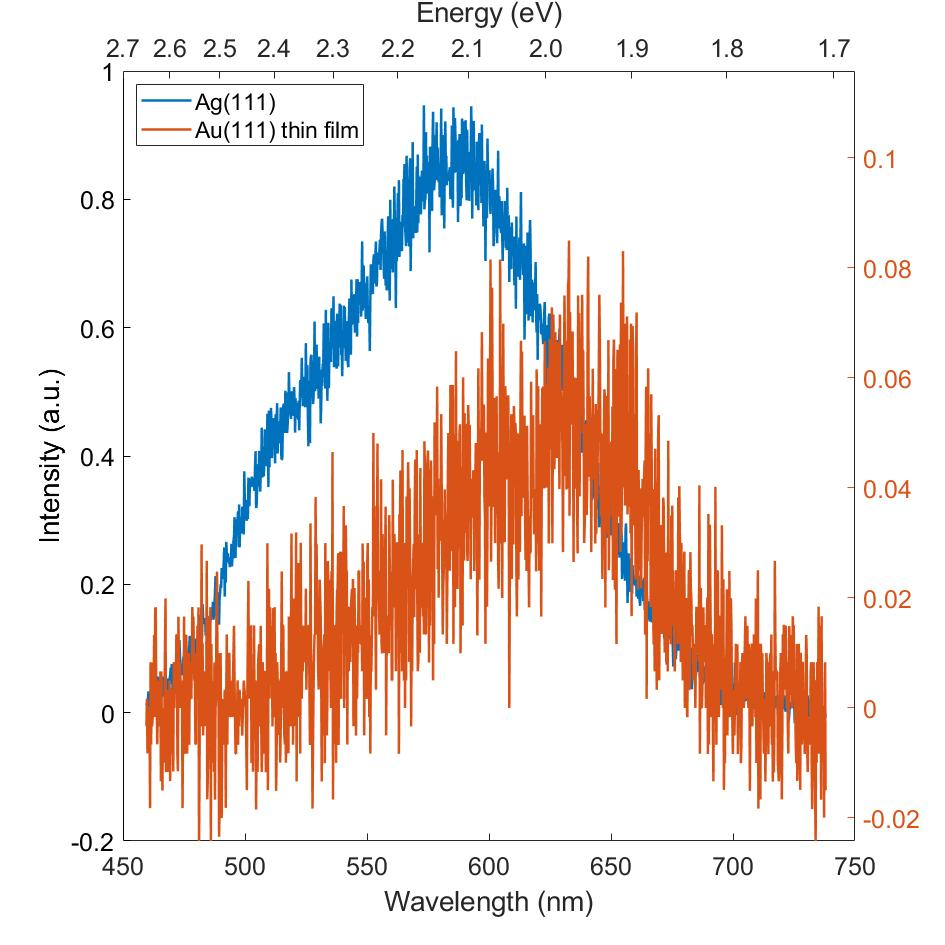
\includegraphics[width=0.6\textwidth]{pictures/Ag_Au_plasmon_3V_200pA_10s.jpg}
    \caption{Plasmonic emission on Ag(111) and Au(111) thin film collected with the same Ag tip (\stmlparams{3}{200}{10}). The signal on the thin film is lower by an order of magnitude, and red-shifted. The Ag(111) emission peaks at \SI{573}{nm}, while the Au(111) emission peaks at \SI{633}{nm}.}
    % 573.3192 Ag, 632.7994 Au
    \label{fig:opv:metal-plasmon}
\end{figure}



When \ac{STML} experiments were carried out on molecular species, the molecules were decoupled by a bilayer (2\ac{ML}) NaCl spacer, which could modify the plasmon emission. Using the same Ag tip, modification of the plasmon emission on Ag(111) by layers of NaCl can be seen in \autoref{fig:opv:nacl-plasmon}. Overall, there was an enhancement in the detected photons when compared to the bare metal substrate.


\begin{figure} [h]
    \centering
    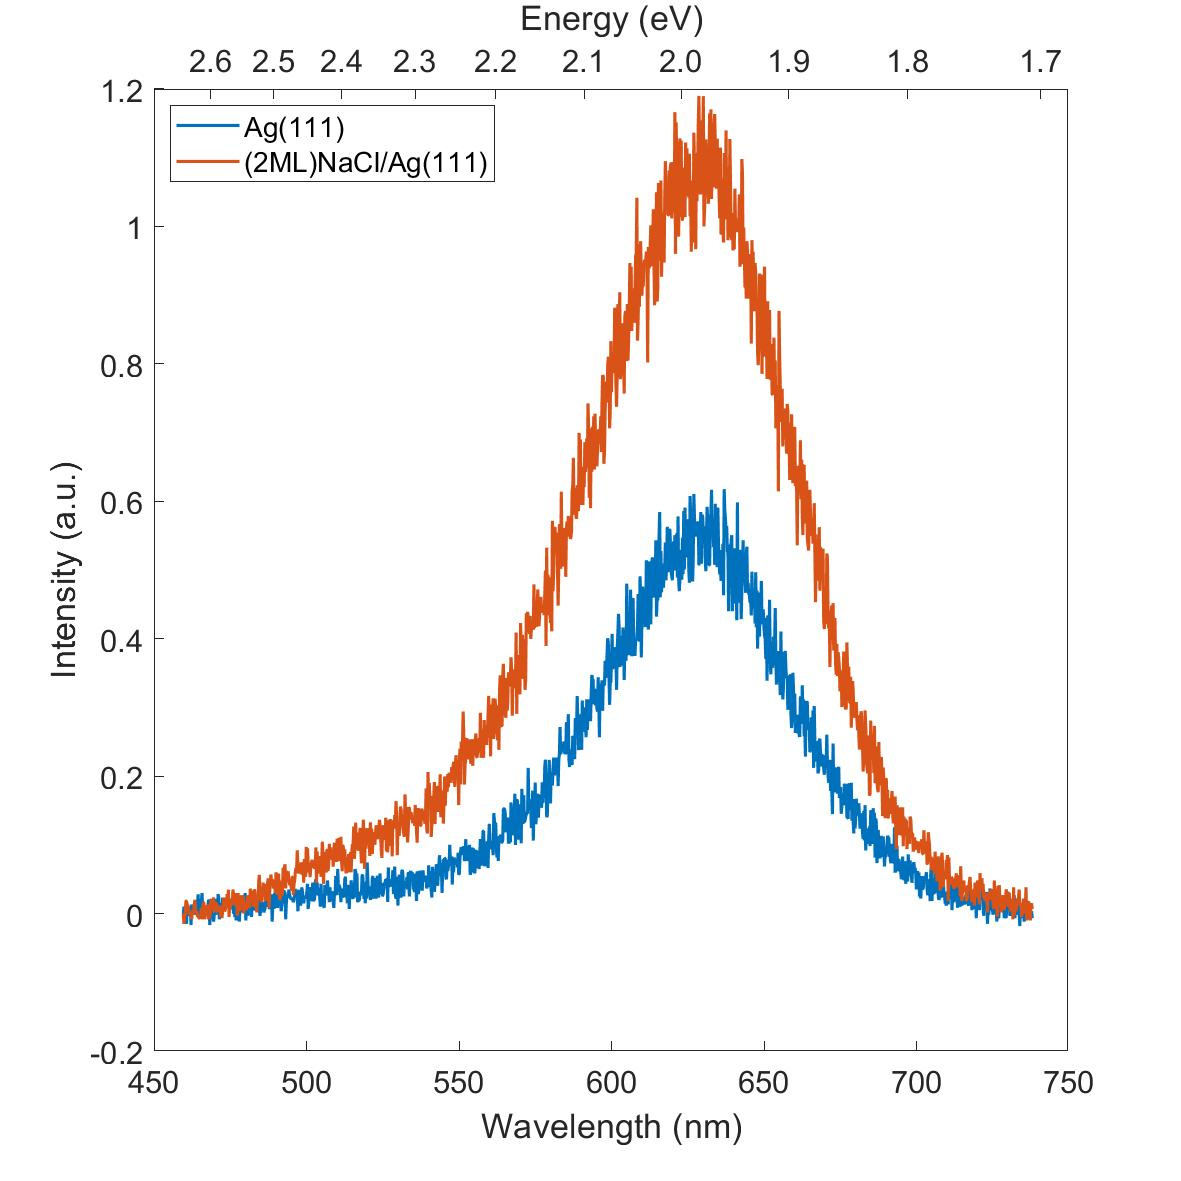
\includegraphics[width=0.6\textwidth]{pictures/NaCl_enhancement_Ag111_275V_250pA_10s.jpg}
    \caption{Plasmonic emission from Ag(111) and on (2ML)NaCl/Ag(111) (\stmlparams{2.75}{250}{10}). There is an enhancement on the bilayer NaCl with minimal shift in energy. }
    % 636.9401 Ag, 628.6561 NaCl/Ag
    \label{fig:opv:nacl-plasmon}
\end{figure}

Thicker layers of NaCl further dissociate the molecule from the metallic substrate, allowing for a more accurate study of the intrinsic properties of the molecule \citep{repp2005molecules}. The thickness of the spacer layer also adjusts the tunnelling rate between the molecule and substrate, changing the rate of charge injection involved in exciton formation. Molecules deposited on thicker layers of NaCl have also demonstrated enhanced molecular luminescence \citep{Zhang2017,Kroger2018}. However, due to the insulating effects of NaCl, the tip-sample distance is smaller for the same bias and setpoint current, resulting in stronger interactions between the tip and the molecule, and affecting the stability of the molecule on the NaCl. Bilayer NaCl gave the most consistent and stable configurations for \ac{STML}.



\section{Study of PTCDA}

Isolated \ac{PTCDA} molecules on (2ML)NaCl/Au(111) were studied with \ac{STML} due to our familiarity with this system. As discussed before, the Au(111) thin film sample is slightly out of focus of the lens, resulting in weaker signals. However, \ac{PTCDA} has a high electron affinity, and the (2ML)NaCl/Ag(111) substrate has a sufficiently low work function that the \ac{LUMO} of PTCDA sits below the Fermi energy of the substrate, resulting in negatively charged PTCDA \citep{cochrane2017single,cochrane2018molecularly}. By using Au(111), which has a higher work function, the PTCDA molecule was not charged on the surface, giving a simpler system to probe. Additionally, previous preliminary work in our group has demonstrated luminescence quenching on the PTCDA/(2ML)NaCl/Ag(111) system \citep{roussy2016coupling}, although a recent publication has shown luminescence at higher biases than had been explored \citep{Kimura2019}.

Luminescence from a single PTCDA on (2ML)NaCl/Au(111) was detected, with an emission peak at \SI{670}{nm} or \SI{1.85}{eV}, at \stmlparams{3}{200}{300} (\autoref{fig:opv:ptcda-stml}). The \ac{FWHM} of the peak is about \SI{90}{meV}, quite broad for single molecule emission. During the acquisition, the PTCDA shifted away, resulting in additional photon counts from the plasmonic emission without the molecule signal present.


\begin{figure} [H]
    \centering
        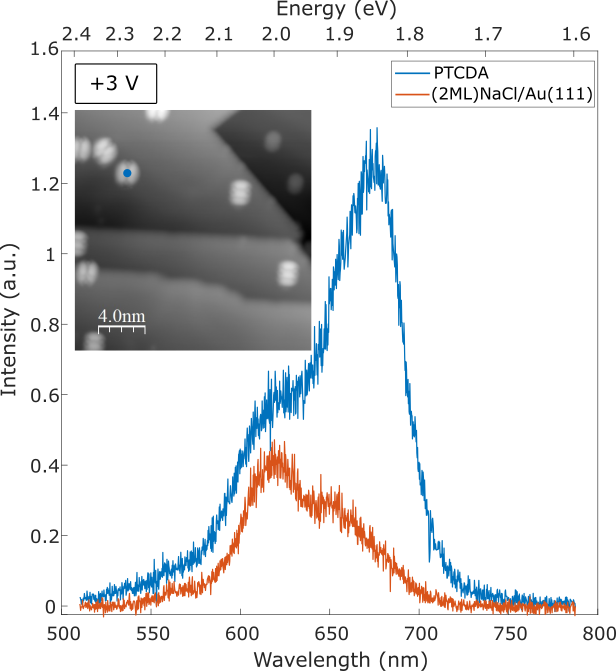
\includegraphics[width=0.6\textwidth]{pictures/ptcda_+ve_emission_inset.png}
    \caption{Luminescence on PTCDA on (2ML)NaCl/Au(111) at positive bias (\stmlparams{3}{200}{300}), with corresponding plasmon on substrate (\stmlparams{3}{200}{30}). Inset is the corresponding STM image with tip position during STML indicated (\stmparams{20}{20}{2}{10}). }
    \label{fig:opv:ptcda-stml}
\end{figure}

We will compare our results to references \citep{Rzeznicka2011} and \citep{Kimura2019}. In the former, \textit{Rze\'znicka et al.} studied self-assembled bilayers of PTCDA on Au(111), with the first monolayer acting as the decoupling layer. The authors reported broad emission peaks at \SI{1.8}{eV} and \SI{2.35}{eV}, with \acp{FWHM} of approximately \SI{100}{meV}, at a bias voltage of \SI{3}{V}. In the latter, \textit{Kimura et al.} studied single negatively charged PTCDA on (3ML)NaCl/Ag(111), detecting a sharp emission peak at \SI{2.45}{eV} at a bias of \SI{-3.4}{V}. 

The peak observed in \autoref{fig:opv:ptcda-stml} most closely resembles the lower energy \SI{1.8}{eV} emission seen by \textit{Rze\'znicka et al.}, who attributed the emission to the \ac{CT} exciton formed between the first and second monolayers of PTCDA. However, our system only consisted of a single isolated PTCDA molecule, with no neighbouring molecules to form a \ac{CT} complex. Additionally, the broadness seen by \textit{Rze\'znicka et al.} could be explained by the effects of adjacent molecules, but our isolated PTCDA system exhibits similar breadth in emissions. Regarding the higher energy photon emission at $\sim$\SI{2.4}{eV}, both publications attributed the emission peak to the $S_1(0) \rightarrow S_0(0)$ exciton recombination. However, we do not see this peak in our experiment, possibly due to the weak plasmonic enhancement in that region of the spectrum.

While the previous references are useful as comparisons, the PTCDA on (2ML)NaCl/Au(111) system studied here was isolated and uncharged. The luminescence observed on this system may be the $S_1(0) \rightarrow S_0(0)$ exciton transition for a neutral PTCDA molecule. Additionally, the luminescence was observed at a high positive bias of \SI{3}{V}. The molecules were noticeably more unstable at positive bias, shifting and rotating during acquisition. It is possible that over the exposure time interval, different vibrational transitions were suppressed and enhanced due to the conformational changes in the molecule, resulting in a shifted and broadened emission peak. 

It is also possible that an alternative mechanism contributed to the emission seen in \autoref{fig:opv:ptcda-stml}, such as the plasmon-mediated exciton formation, or charge injection into LUMO+1 of PTCDA. While there remain open questions about the emission seen on PTCDA, due to stability issues, further experiments were not performed. A more thorough investigation of the shifted and broadened emission at positive biases is required to fully understand the signal observed.



\section{Study of {ZnPc}}

\ac{ZnPc} is a relatively planar organic semiconducting molecule that can be thermally deposited, making it optimal for \ac{SPM} study. To maximize \ac{STML} signal, ZnPc was deposited on (2ML)NaCl/Ag(111) and probed with the Ag tip. With parameters \stmlparams{3}{300}{300}, we were able to detect an emission peak from ZnPc at \SI{630}{nm} or \SI{1.96}{eV} (\autoref{fig:opv:znpc-stml}).

% Because of previous reports of \ac{STML} on ZnPc, this molecule was used to test the \ac{STML} capabilities of our system. 

% The structure of the ZnPc is shown in \autoref{fig:opv:znpc-stm}. The substrate was (2ML)NaCl/Au(111) thin film, and the tip used was the Pt/Ir tip dipped in gold. At biases higher than \SI{1}{V}, the ZnPc molecule rotates to give a 16-lobed structure. The non-rotating molecule has an 8-lobed structure, which could be seen if the molecules were ``anchored" by some defect or step edge, or was dimerized to another molecule.  

% \begin{figure} [h]
%     \centering
%     %\includegraphics[width=3in]{file}
%     \caption{\FIXME{Show stm of ZnPc (-1V, 1.0, 2.0), also with dimerize }}
%     \label{fig:opv:znpc-stm}
% \end{figure}

% The electronic structure was then probed using \ac{STS}. The \ac{LDOS} along with the molecular orbitals at the resonances are shown in \autoref{fig:opv:znpc-sts}.

% \begin{figure} [h]
%     \centering
%     %\includegraphics[width=3in]{file}
%     \caption{\FIXME{Show sts of ZnPc on Au(111)}}
%     \label{fig:opv:znpc-sts}
% \end{figure}

% Previous reports of ZnPc on this substrate show that the electronic states of the molecule do not change much in structure, and only experience a rigid shift of $\approx \SI{-1}{eV}$ in energy when compared to (2ML)NaCl/Au(111), due to the lower work function of (2ML)NaCl/Ag(111) \citep{Doppagne2017,Doppagne2018}. With an optimized Ag tip, photoluminescence was detected on the molecule, with an emission peak at \SI{630}{nm} or \SI{1.96}{eV} (\autoref{fig:opv:znpc-stml}).

                    

\begin{figure} [H]
    \centering
    
        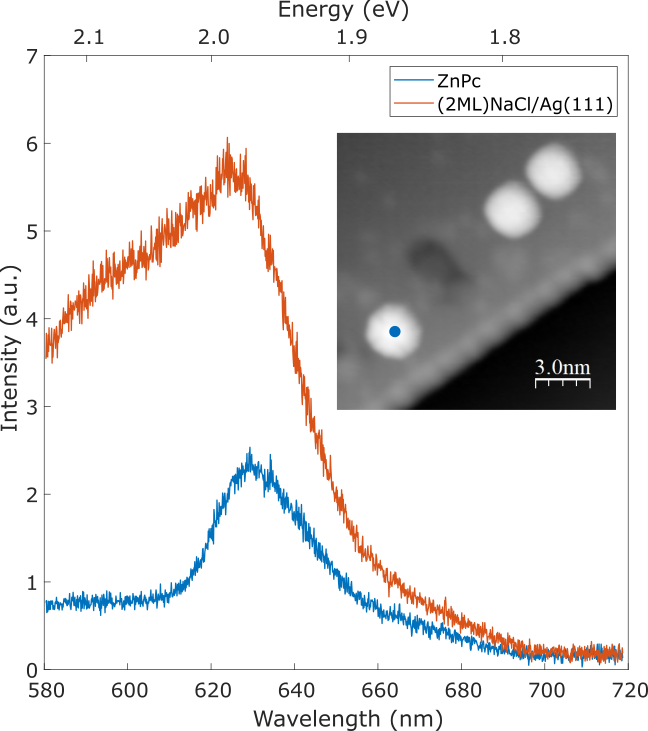
\includegraphics[width=0.6\textwidth]{pictures/znpc_+ve_emission_inset.png}
    
    \caption{Luminescence on ZnPc on (2ML)NaCl/Ag(111) at positive bias, with corresponding plasmon on substrate. Both spectra were taken at \stmlparams{3}{300}{300}. Inset is the corresponding STM image with tip position during STML indicated (\stmparams{15}{15}{2}{10}). }
    \label{fig:opv:znpc-stml}
\end{figure}

There are notable differences between our results and the results of past reports of \ac{STML} on ZnPc \citep{Zhang2016, Doppagne2017, Zhang2017, Doppagne2018}. An example of ZnPc \ac{STML} spectra from the literature is provided in \autoref{fig:opv:znpc_literature}. The previously reported main emission peak was at \SI{652}{nm} or \SI{1.9}{eV}. This peak was attributed to the $S_1(0) \rightarrow S_0(0)$ transition in ZnPc. The peak energy in \autoref{fig:opv:znpc-stml} is higher in energy, and about four times broader, with \ac{FWHM} of about \SI{60}{meV} while previously reported emissions have \ac{FWHM} of about \SI{15}{meV}.

\begin{figure}
    \centering
    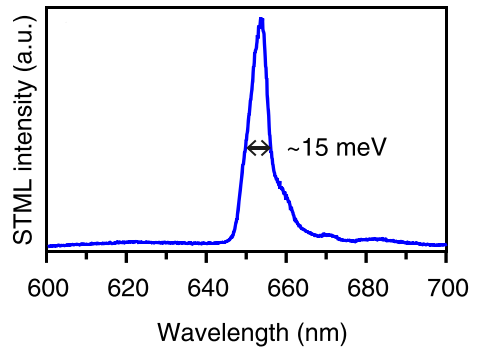
\includegraphics[width=0.4\textwidth]{pictures/znpc_literature.PNG}
    \caption[Luminescence on ZnPc on (2ML)NaCl/Ag(111) at negative bias. Spectra was taken at \stmlparams{-2.5}{200}{20}. The emission peak is at \SI{653}{nm}, and the FWHM is \SI{15}{meV}. ]{Luminescence on ZnPc on (2ML)NaCl/Ag(111) at negative bias. Spectra was taken at \stmlparams{-2.5}{200}{20}. The emission peak is at \SI{653}{nm}, and the FWHM is \SI{15}{meV}. Figure taken from \citep{zhang2017sub}.}
    \label{fig:opv:znpc_literature}
\end{figure}

% The shift in energy and broadening of the molecular photoluminescence may be a result of the IR filters in place during our experiments. All \ac{STML} data was taken with the KG5 infrared filters in place, which have a transmittance cutoff in the range of the emission seen in \autoref{fig:opv:znpc-stml}. At around \SI{650}{nm}, the transmittance drops significantly to 50\% (\autoref{fig:expsetup:windows}), resulting in blue-shift and broadening of our signal. 

In contrast to past reported results taken at \SI{-2.5}{V}, we detected luminescence at a tip-sample bias of \SI{3}{V}. ZnPc has two equivalently stable adsorption angles on NaCl \citep{Miwa2016}, and rapid shuttling between these geometries has been observed. Similar to PTCDA, the ZnPc was noticeably more unstable at high positive biases, rotating and shifting more frequently, seen as sub-\AA ngstr\"om jumps in the tip height. This instability can change the vibrational transitions of the ZnPc observed in the luminescence, shifting and broadening the emission signal in \autoref{fig:opv:znpc-stml}. Another factor that may explain the discrepancies observed is the presence of an alternative mechanism of molecular luminescence. The luminescence seen at positive bias may be a result of plasmon-mediated exciton recombination or some other molecular luminescence mechanism.


%Studies in the literature on \ac{STML} on ZnPc have described the emission to be the recombination of excitons formed by charge injection. However, at positive biases, charge injection exciton formation would require the Fermi level of the metal substrate to fall below the energy of the \ac{HOMO} of ZnPc in order to inject a hole into the system. Such a large shift is unlikely at a modest bias of \SI{3}{V}, and so t








% A recent work by \emph{Kimura et al.} was the first report of single molecule \ac{STML} on a negatively charged PTCDA, with a substrate of (3ML)NaCl/Ag(111). The authors corresponded the $S$ \FIXME{notation for the franck condon transitions} transition to an emission peak at \SI{2.45}{eV} with bias onset at $V_b=\SI{-2.2}{V}$ \citep{Kimura2019}. The energy of the emission peak seen in \autoref{fig:opv:ptcda-stml} does not correspond to

% Additionally, our detected emission is broadened, with a \ac{FWHM} of \SI{100}{meV}. The broadness and energy is similar to the \ac{CT} emission seen on the bilayer system, however, there were no neighbouring molecules in our system to broaden the signal or to form a \ac{CT} state. 

% An earlier study looked at \ac{STML} on a bilayer of \ac{PTCDA}, with the first monolayer acting as the decoupling layer. The authors found a broad \ac{CT} emission at \SI{1.75}{eV} for $V_b =\SI{2.5}{V}$, and an additional weaker $S_{10}$ transition at \SI{2.35}{eV} for $V_b = \SI{3.0}{V}$ \citep{Rzeznicka2011}. 

% A possible explanation for our spectra in \autoref{fig:opv:ptcda-stml} is the tunnelling






\section{Study of \ch{F8ZnPc}}

The energy of molecular orbitals can be tuned through halogenation, such as the introduction of fluorine into a molecular structure. Studies of fluorination on organic molecule films have demonstrated a rigid downward shift in energy of the HOMO and LUMO states, effectively raising the Fermi level \citep{schwarze2016band,warren2019controlling}. Using \ac{SPM}, the effects of fluorination could be understood at the single molecule level. 

\subsection{Comparison of STM/STS of ZnPc and \ch{F8ZnPc}}

ZnPc and \ch{F8ZnPc} were co-deposited on (2ML)NaCl/Au(111), and STM and STS was conducted using a Pt/Ir tip (\autoref{fig:opv:fluorination_shift}). In the topography, the effects of fluorination on the adsorption geometry of the molecule is immediately obvious. ZnPc on bilayer NaCl appears 16-lobed, as it shuttles between two equally stable adsorption angles, agreeing with past \ac{STM} studies of ZnPc \citep{Miwa2016, Imada2016}. The fluorines in \ch{F8ZnPc} ``anchor" and stabilize the molecule on the NaCl, giving an 8-lobed structure in the STM topography. The effects of the fluorination on the adsorption geometry of the molecule will be discussed in detail in \autoref{sec:opv:adsorp}. 


\begin{figure} [H]
    \centering
        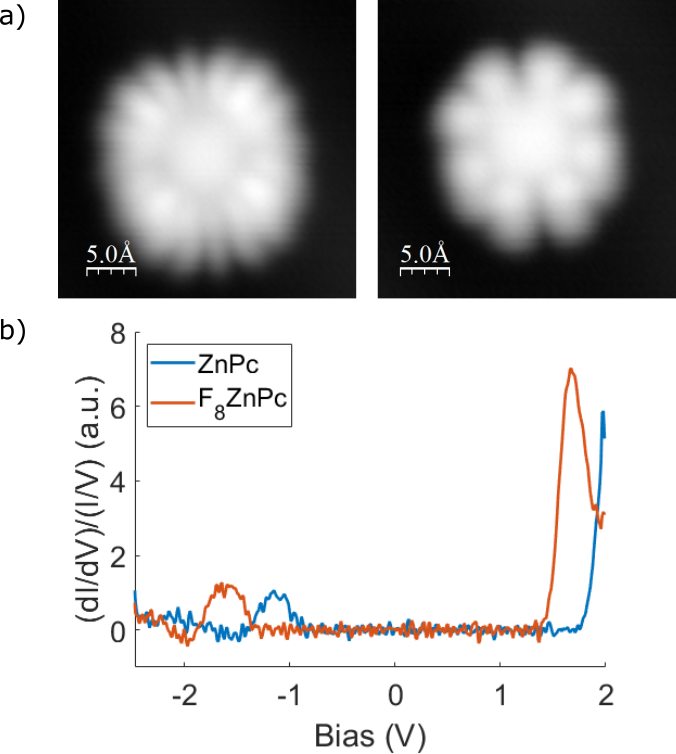
\includegraphics[width=0.6\textwidth]{pictures/znpc_f8znpc_comparison.png}
    \caption{ STM and STS data of ZnPc and \ch{F8ZnPc} on (2ML)NaCl/Au(111). \textbf{(a)} STM images of ZnPc and \ch{F8ZnPc} (\stmparams{3}{3}{-2.5}{5}). \textbf{(b)} Normalized $dI/dV$ of ZnPc and \ch{F8ZnPc} on (2ML)NaCl/Au(111).  }
    \label{fig:opv:fluorination_shift}
\end{figure}

\ac{STS} reveals a downward shift of about \SI{0.49}{eV} in the HOMO state onset and about \SI{0.41}{eV} in the LUMO state onset of \ch{F8ZnPc} relative to the states of ZnPc (\autoref{fig:opv:fluorination_shift}b), resulting in a \SI{0.09}{eV} widening of the band gap due to fluorination of ZnPc. This result differs slightly from the rigid shift observed in mixed films of fluorinated and non-fluorinated ZnPc \citep{schwarze2016band}, likely due to the differences in configuration and local environment of the molecules between the experiments.

% The shifting of molecular states through fluorination has applications to heterojunction design in \ac{OPV} devices. Further \ac{STS} and \ac{STML} experimentation on the ZnPc/\ch{F8ZnPc} heterodimer may reveal the effects of the heterojunction on charge transfer and exciton recombination at the single molecule level.

\subsection{Luminescence on \ch{F8ZnPc}}

\ch{F8ZnPc} was thermally deposited onto (2ML)NaCl/Ag(111) and probed with a Ag tip. With positive bias \stmlparams{3}{250}{60}, a weak emission peak was detected at \SI{675}{nm} or \SI{1.83}{eV}, with FWHM of approximately \SI{40}{meV} (\autoref{fig:opv:f8znpc-stml_+}). 
% Using previously observed photoluminescence of ZnPc as an estimate, the tip plasmon was tuned to enhance primarily in the region of \SI{630}{nm}. 

\begin{figure} [H]
    \centering
        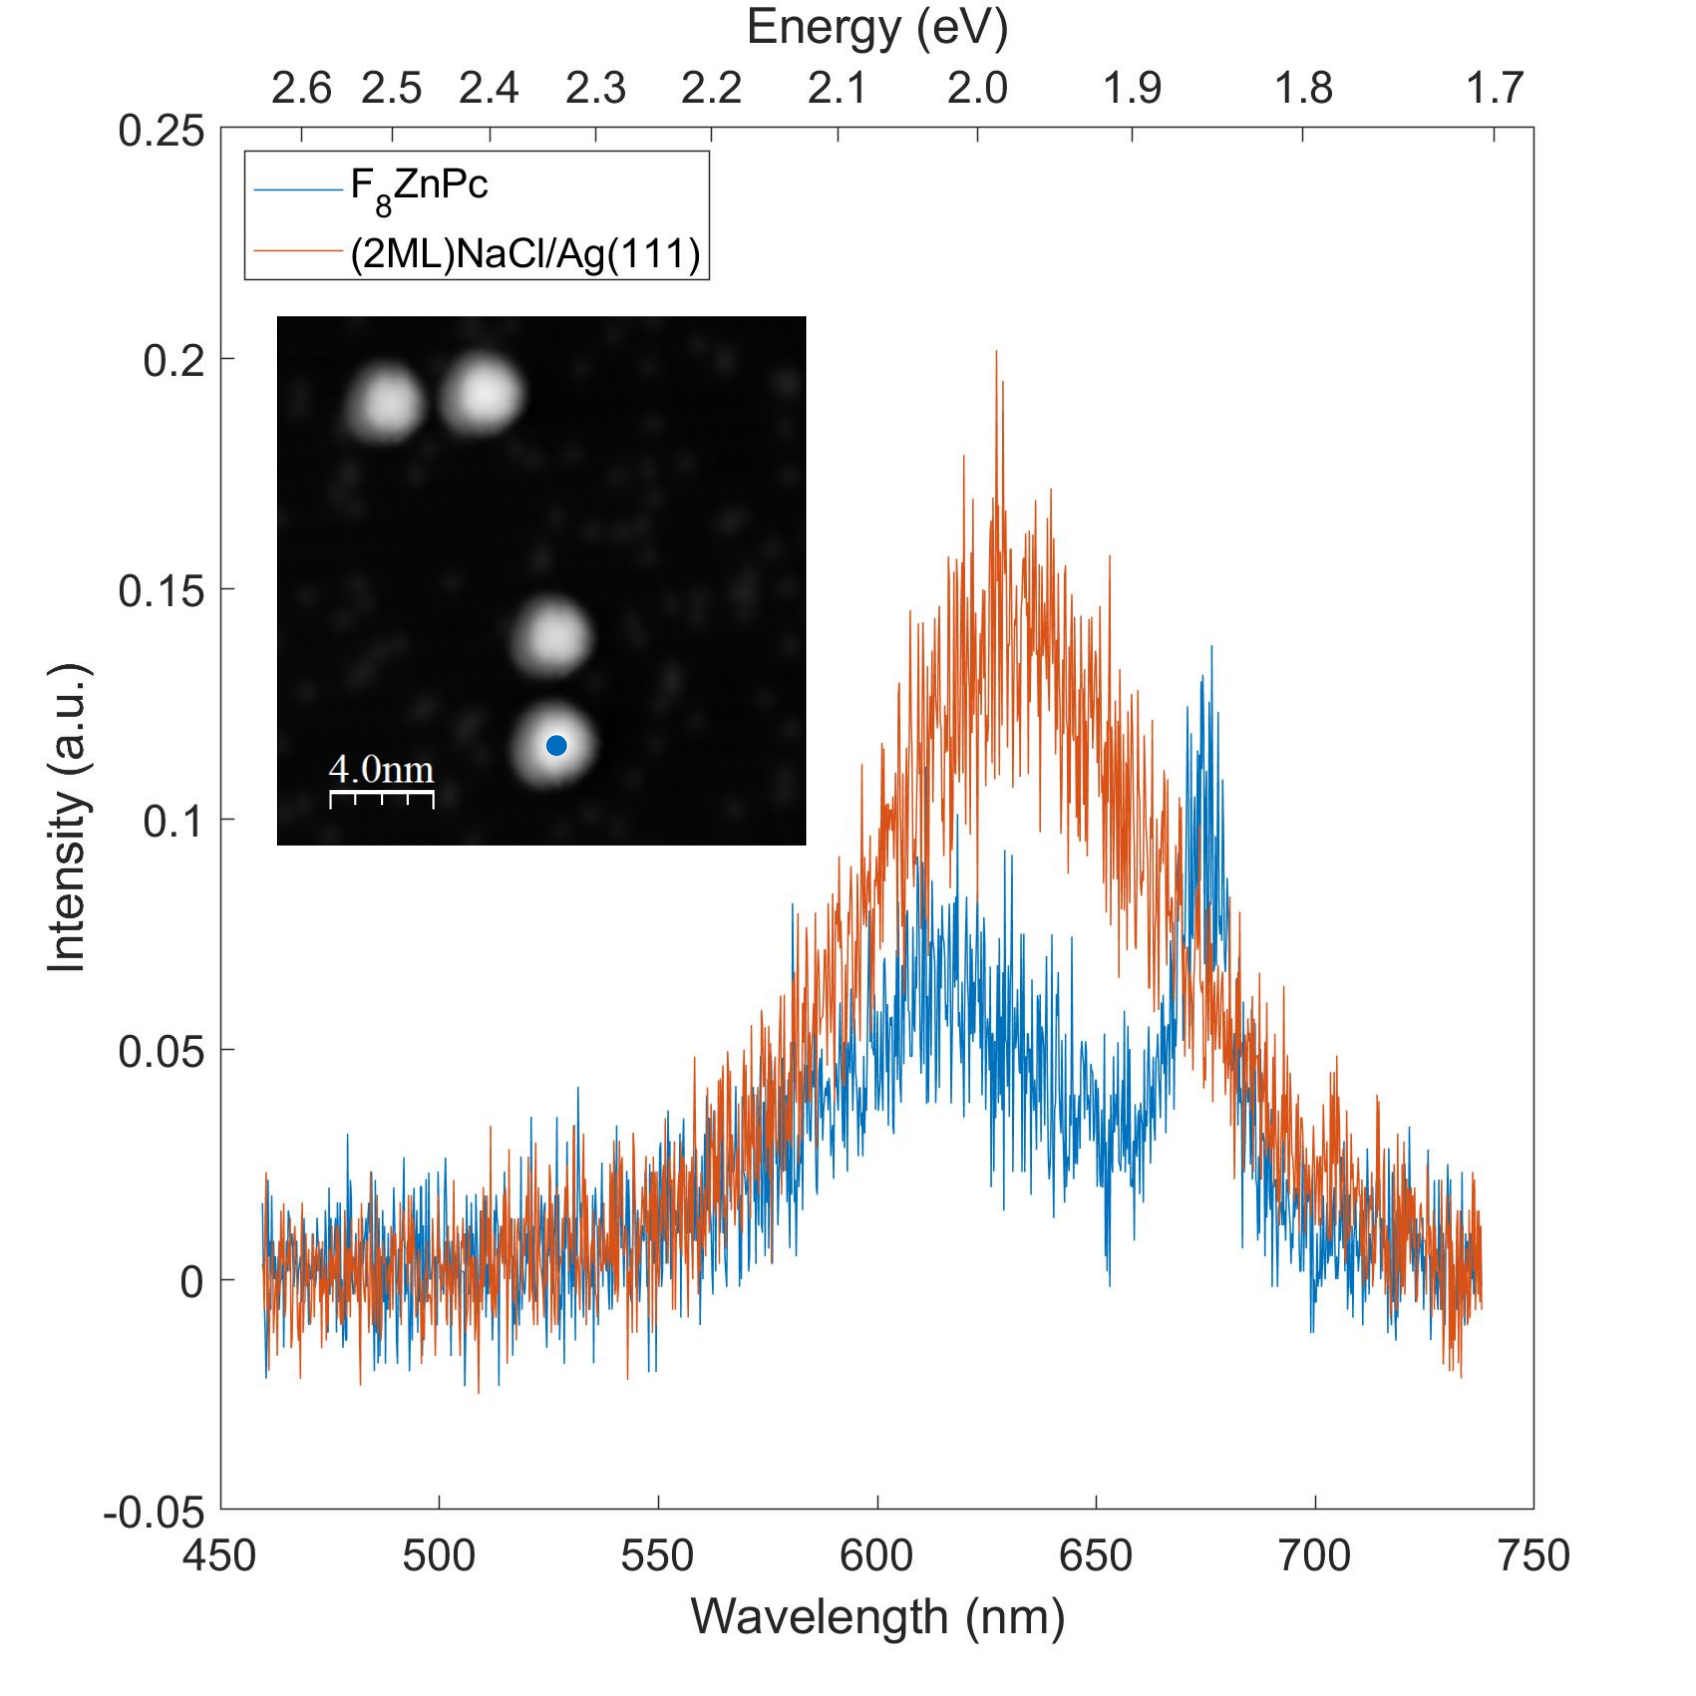
\includegraphics[width=0.6\textwidth]{pictures/f8znpc_+ve_emission_inset.png}
    \caption{Luminescence on \ch{F8ZnPc} on (2ML)NaCl/Ag(111) at positive bias (\stmlparams{3}{250}{60}), with corresponding plasmon on substrate (\stmlparams{3}{250}{10}). A peak is observed at \SI{675}{nm}. Inset is the corresponding STM image with tip position during STML indicated (\stmparams{20}{20}{2}{10}). }
    \label{fig:opv:f8znpc-stml_+}
\end{figure}

When compared to the positive emission on ZnPc (\autoref{fig:opv:znpc-stml}), the emission in \autoref{fig:opv:f8znpc-stml_+} is slightly sharper, possibly due to the stabilizing effect of the fluorine atoms in \ch{F8ZnPc}. However, shifts and rotations of \ch{F8ZnPc} were observed during positive bias \ac{STML}, broadening the emission relative to negative bias emissions seen in previous studies on ZnPc (\autoref{fig:opv:znpc_literature}). Additionally, the positive bias emission peak on \ch{F8ZnPc} is red-shifted by about \SI{45}{nm} when compared to that of the ZnPc, but without further knowledge of the vibrational transitions involved in the positive bias emission, quantitative comparisons between the emissions cannot be made.

\ac{STML} was also conducted at negative bias for \ch{F8ZnPc}, and luminescence was detected at \stmlparams{-2.5}{200}{120}. A strong and sharp $S_1(0) \rightarrow S_0(0)$ emission peak was observed at \SI{640}{nm} or \SI{1.93}{eV}, along with well-resolved satellite peaks corresponding to vibrational transitions (\autoref{fig:opv:f8znpc-stml_-}). The \ac{FWHM} is approximately \SI{20}{meV}, comparable to the negative bias emissions observed on ZnPc. 


\begin{figure} [H]
    \centering
           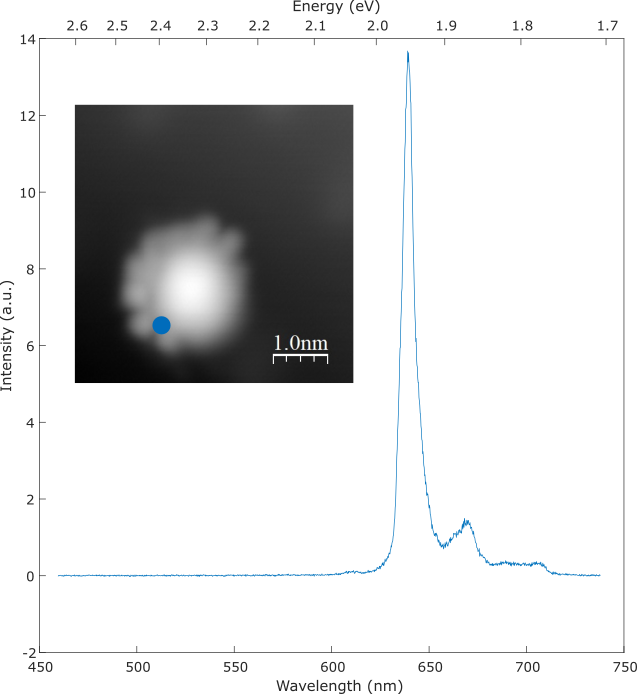
\includegraphics[width=0.6\textwidth]{pictures/f8znpc_-ve_emission_inset300.png}
        \caption{Luminescence at negative bais detected on \ch{F8ZnPc} on (2ML)NaCl/Ag(111) with 300 gr/mm grating (\stmlparams{-2.5}{200}{120}). Peak detected at \SI{640}{nm}, with lower energy vibrational peaks. Inset is the corresponding STM image with tip position during STML indicated (\stmparams{5}{5}{-2}{10}).}
        \label{fig:opv:f8znpc-stml_-}
\end{figure}

When compared to the positive bias emission in \autoref{fig:opv:f8znpc-stml_+}, the negative bias emission is blue-shifted by \SI{35}{nm}. A broad vibrational peak in the negative bias emission in \autoref{fig:opv:f8znpc-stml_-} coincides at the energy of around \SI{670}{nm}---the same energy as the positive bias emission peak in \autoref{fig:opv:f8znpc-stml_+}---providing supporting evidence that lower energy vibrational transitions were responsible for the observations in the positive bias \ac{STML} experiments.  Due to complications involving the shifting and broadening of spectral features due to different adsorption geometries and stability of the molecules at positive bias, further positive bias \ac{STML} investigation is required to determine the source and mechanism of the emission.

When compared to published negative bias \ac{STML} data on \ac{ZnPc} (\autoref{fig:opv:znpc_literature}), the emission peak on \ch{F8ZnPc} in \autoref{fig:opv:f8znpc-stml_-} is slightly higher in energy by about \SI{0.03}{eV}. This suggests a widening of the optical gap, corresponding to an asymmetric shift of the HOMO and LUMO states due to fluorination of ZnPc, widening the band gap of the molecule. The change in the optical gap is in accordance with the change in the band gap seen in \ac{STS} of the ZnPc and \ch{F8ZnPc} (\autoref{fig:opv:fluorination_shift}).  Local environment, adsorption geometry, and molecule-substrate interactions may affect the energy levels of \ch{F8ZnPc}; this is explored in detail in \autoref{sec:opv:adsorp}.

Higher resolution spectra were obtained with the 600 gr/mm grating to better resolve the vibrational emission peaks (\autoref{fig:opv:f8znpc-stml_600gr}). With the tip positioned above different parts of the molecule, changes in the lower energy vibrational satellite peaks were observed due to different preferred transitions between the excited $S_1$ state and the vibrational states of $S_0$. Sub-molecular location dependent emission from vibrational transitions has been reported before on ZnPc \citep{Zhang2016,Doppagne2017}. Shifts in the energy of the main $S_1(0) \rightarrow S_0(0)$ transition were minimal ($\sim \pm \SI{1}{nm}$). The strongest emission was observed with the tip positioned above the lobes of \ch{F8ZnPc}, and so all further experiments were performed at this location for maximal signal strength.


\begin{figure}[H]
    \centering
        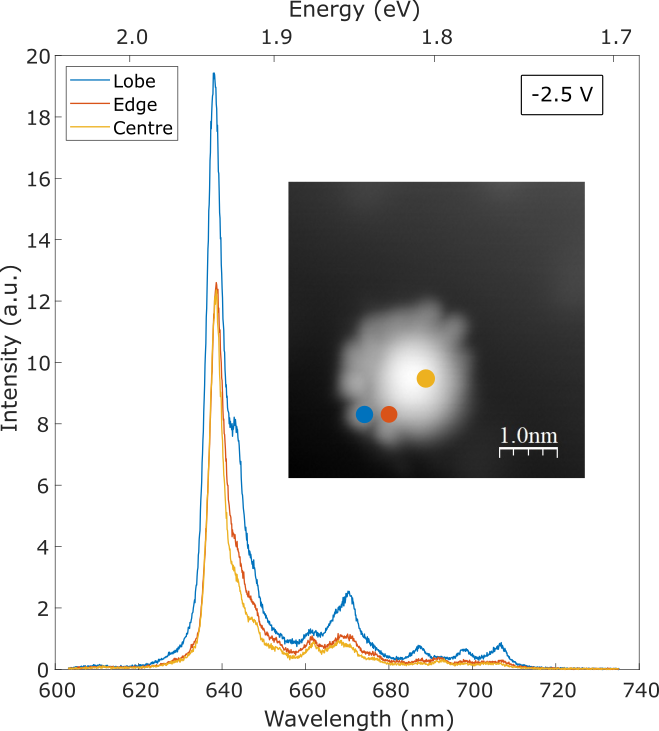
\includegraphics[width=0.6\textwidth]{pictures/f8znpc_-ve_emission_inset600_position.png}
        \caption{Changes in vibrational satellite peaks as the tip is positioned over different parts of \ch{F8ZnPc} on (2ML)NaCl/Ag(111) with 600gr/mm grating. STML parameters were \stmlparams{-2.5}{100}{300} for each point. Inset is the corresponding STM image with tip position during STML indicated (\stmparams{5}{5}{-2}{10}).}
        \label{fig:opv:f8znpc-stml_600gr}
\end{figure}



\subsubsection*{Diversity in molecular types}

% introduce the different species problem

Surprisingly, the \ac{STM} scans at negative biases revealed a variety of topographically different molecules on the surface that were not previously evident at positive biases. To eliminate the possibility of fragmentation or degradation of molecules, a new sample of \ch{F8ZnPc} was loaded into the evaporator crucible, and the sample was prepared again. However, the same diversity was still present (\autoref{fig:opv:f8znpc-stm_diff}). Additionally, we were able to induce switching from one type to another with the tip, suggesting differences in the interaction between molecule and substrate as the cause for the distinct types. Possible reasons include the presence of defects or contaminants, and adsorption geometry of \ch{F8ZnPc} on the substrate.


\begin{figure} [H]
    \centering
    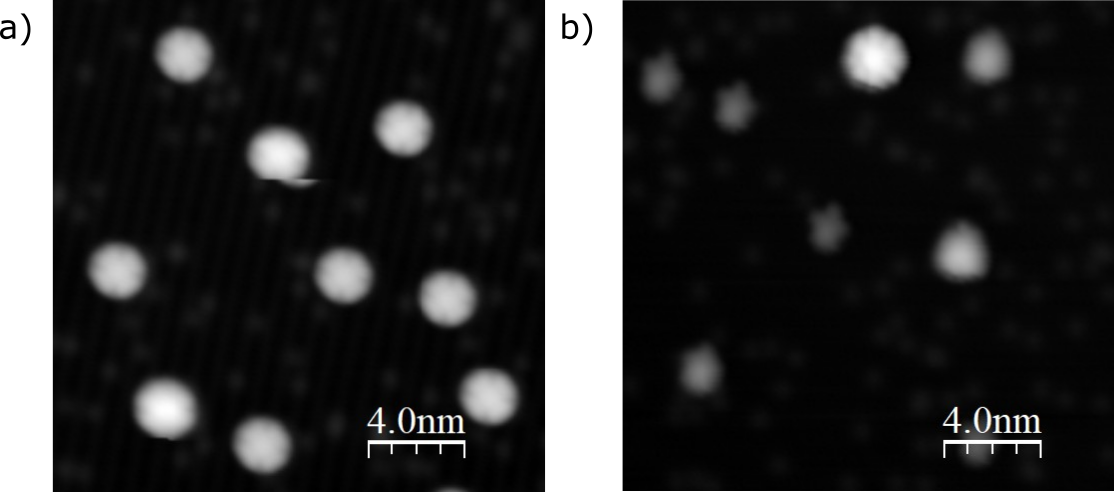
\includegraphics[width=\textwidth]{pictures/diversity.png}
    \caption{Same sample of \ch{F8ZnPc} on (2ML)NaCl/Ag(111) scanned at positive and negative biases. \textbf{(a)} STM image at \stmparams{20}{20}{2}{5}. All molecules appear similar. The striped Moir\'e pattern between NaCl(001) and Ag(111) lattices can be observed. \textbf{(b)} STM image at \stmparams{20}{20}{-2}{5}. Same sample of molecules showing diversity in topography at negative bias. }
    \label{fig:opv:f8znpc-stm_diff}
\end{figure}

Further \ac{STML} experiments at negative biases were conducted on the different types of \ch{F8ZnPc}, with $S_1(0) \rightarrow S_0(0)$ transition peaks varying in wavelengths from \SI{630}{nm} to \SI{643}{nm}. In order to relate the emission peaks to the electronic states of the molecules, \ac{STML} along with \ac{STS} was performed on three of the observed types (\autoref{fig:opv:f8znpc-sts_stml}). 


\begin{figure} [H]
    \centering
        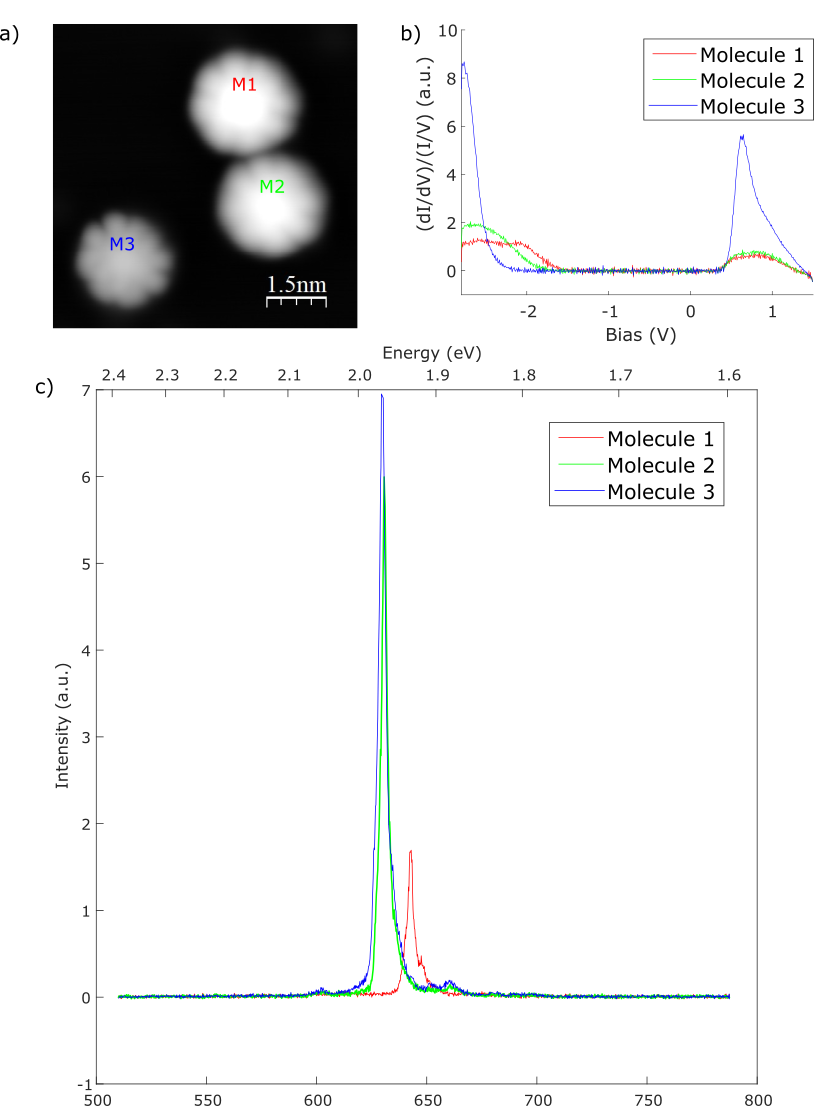
\includegraphics[width=0.7\textwidth]{pictures/3species_diagram.png}
        \caption{STM, STS and STML of 3 types of \ch{F8ZnPc} observed on (2ML)NaCl/Ag(111). \textbf{(a)} Three molecules labelled in STM image (\stmparams{7.5}{7.5}{-2.7}{10}). \textbf{(b)} Normalized $dI/dV$ of each molecule. \textbf{(c)} Luminescence of each molecule taken at \stmlparams{-2.5}{100}{120}. }
    \label{fig:opv:f8znpc-sts_stml}
\end{figure}


With increasing band gaps, measured as the difference in onset energy of HOMO and LUMO, there is a corresponding increase in the optical gaps, observed as higher energy $S_1(0) \rightarrow S_0(0)$ emission peaks from exciton recombination. The results are tabulated in \autoref{tab:opv:bandgaps_3species}. Further experimentation on this sample was not attempted due to the unstable nature of the Ag tip, making it unsuitable for high resolution \ac{STM} or \ac{STS}, and also the wide variety of types of \ch{F8ZnPc} observed on the surface.
 
 \begin{table}[H]
\begin{center}
    \begin{tabular}{|c|c|c|} 
    \hline
        Type  & STS band gap (eV)  &  STML optical gap (eV) \\
        \hline
        Molecule 1  &    2.00   & 1.94   \\
        Molecule 2  &    2.32   & 1.96 \\
        Molecule 3  &    2.75   & 1.97 \\
        \hline
    \end{tabular}
    \caption{Table of band and optical gaps of three types of \ch{F8ZnPc} on (2ML)NaCl/Ag(111), extracted from STS and STML experiments respectively.}
    \label{tab:opv:bandgaps_3species}
    \end{center}
\end{table}


\subsection{Adsorption geometry of \ch{F8ZnPc}}
\label{sec:opv:adsorp}

To further investigate the adsorption geometry of \ch{F8ZnPc} on the substrate, the same sample was prepared after a full system vent and bake-out to ensure all contaminants in the chambers were purged.\footnote{It was during this time that the new windows were installed (\autoref{fig:expsetup:windows}).} The Pt/Ir tip was used for consistent \ac{STM} and \ac{STS} of the \ch{F8ZnPc} on (2ML)NaCl/Ag(111). Despite the same sample preparation conditions, there were clear differences between the sample used for \ac{STML} experiments, and the sample used for investigating the adsorption geometry of \ch{F8ZnPc}. The insulating NaCl layers had a lower density of defects, and there were fewer types of \ch{F8ZnPc} after deposition, making classification more manageable. This suggests that some of the molecular variety may have been the result of underlying defects. 

% It was during this time that the new windows were installed (\autoref{fig:expsetup:windows}), but, due to time constraints, no additional \ac{STML} experiments were carried out.

%\footnote{I will distinguish to the two samples by referring to them as pre- and post-bakeout, respectively.}


\begin{figure} [H]
    \centering
        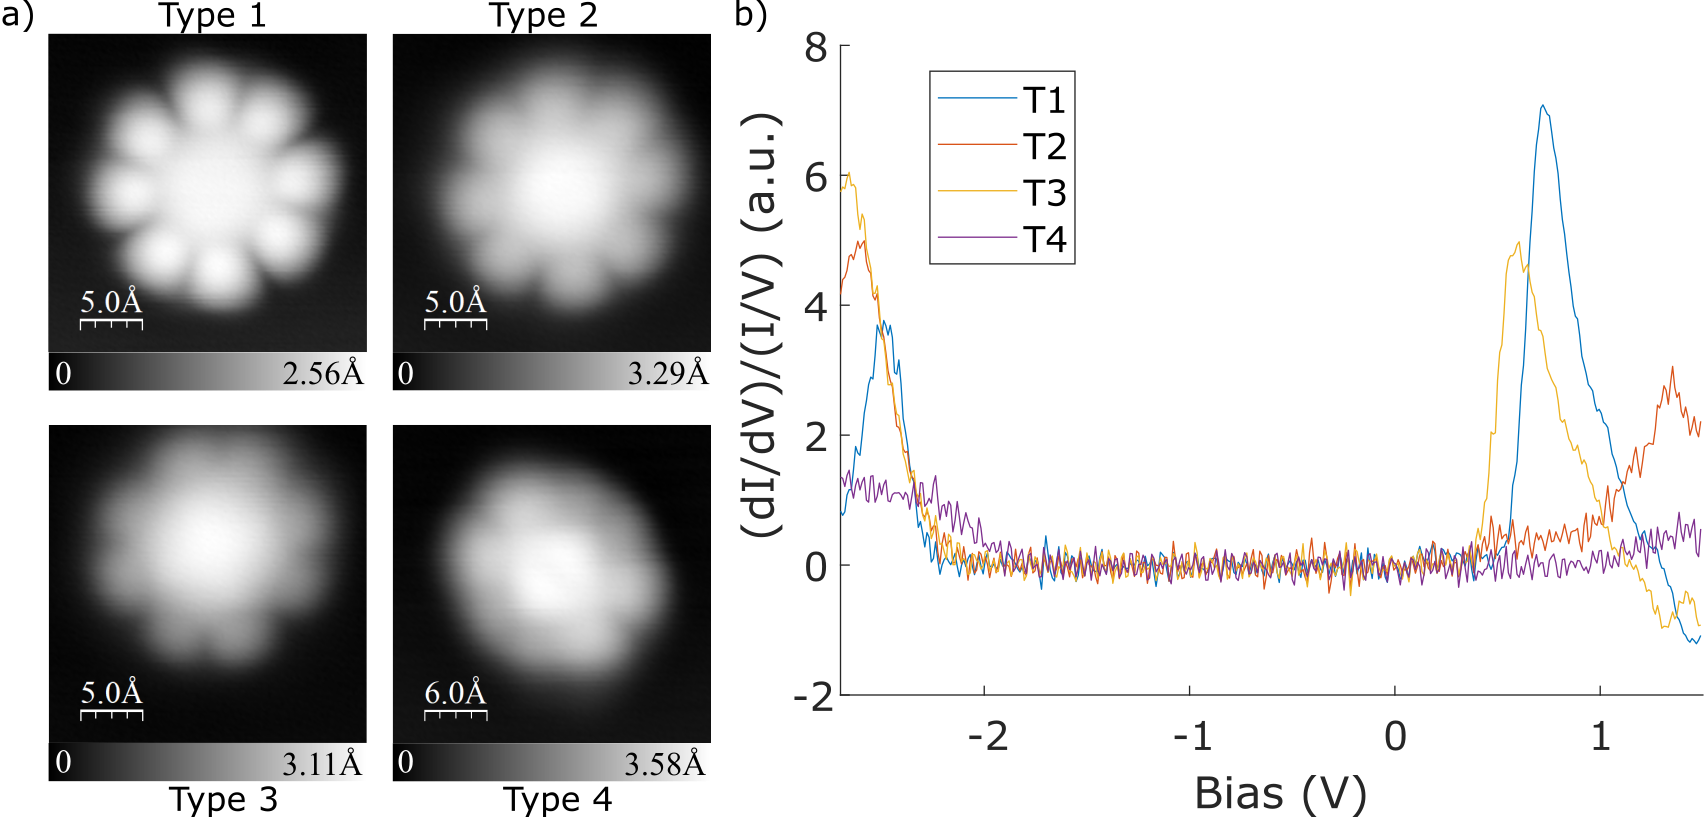
\includegraphics[width=\textwidth]{pictures/4types_images.png}
    \caption{The four identified types of \ch{F8ZnPc} on (2ML)NaCl/Ag(111). \textbf{(a)} STM images of the four types ($V_b = -2.5V$ and $I_t = 5pA$). STM of types 1--3 are \SI{2.5x2.5}{nm}, while type 4 is \SI{3x3}{nm}. \textbf{(b)} Normalized $dI/dV$ from point STS taken on each of the four types. }
    \label{fig:opv:f8znpc-sts_types}
\end{figure}

Nevertheless, we identified four main types of \ch{F8ZnPc}, each with distinct topography and \ac{STS} resonances, as seen in \autoref{fig:opv:f8znpc-sts_types}. The types were named in order of most to least abundant: T1, T2, T3, and T4. The band gaps changed with each molecule type, as observed in the sample used for \ac{STML}. The band gaps, measured from the onsets of HOMO and LUMO states, for each molecule type are summarized in \autoref{tab:opv:bandgaps_4types}. There were additional types, but, due to rarity and molecular instability, they were not classified or examined in depth. 

\begin{table}[H]
\begin{center}
    \begin{tabular}{|c|c|} 
    \hline
        Type  & STS band gap (eV) \\
        \hline
        T1  &    2.75  \\
        T2  &    2.58  \\
        T3  &    2.55\\
        T4  &    3.01\\
        \hline
    \end{tabular}
    \caption{Table of band gaps of the four types of \ch{F8ZnPc} on (2ML)NaCl/Ag(111), extracted from STS experiments.}
    \label{tab:opv:bandgaps_4types}
    \end{center}
\end{table}

Furthermore, the configuration of each type of \ch{F8ZnPc} relative to the underlying NaCl lattice was examined. For each molecule type, the surrounding NaCl was scanned with high current and low bias to give atomic resolution of the NaCl lattice, as seen in \autoref{fig:exptech:stmexample}. The scanning parameters were then restored when scanning over the molecule. The lattice was then extended for the entire image, with the bright atoms corresponding to \ch{Cl-} ions \citep{heidorn2013influence}. The results for each type of \ch{F8ZnPc} are summarized in \autoref{fig:opv:f8znpc-atomic_types}.

\begin{figure} [h]
    \centering
        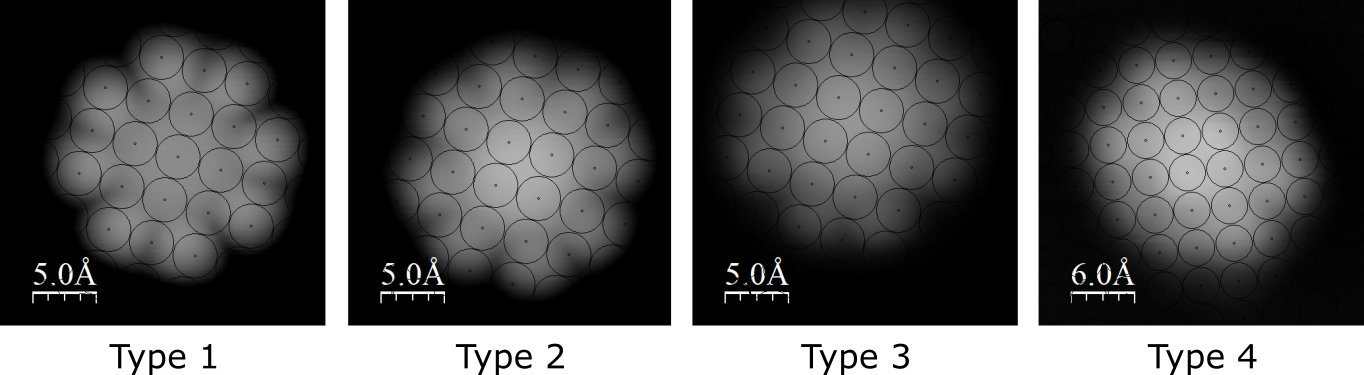
\includegraphics[width=\textwidth]{pictures/4types_atomic.png}
    \caption{STM images of four identified types of \ch{F8ZnPc} on (2ML)NaCl/Ag(111) with underlying NaCl lattice superimposed ($V_b = -2.5V$ and $I_t = 5pA$). The circles indicate the \ch{Cl-} ion. Types 1--3 are \SI{2.5x2.5}{nm}, while type 4 is \SI{3x3}{nm}.  }
    \label{fig:opv:f8znpc-atomic_types}
\end{figure}

In the T1 configuration, \ch{F8ZnPc} has a 4-fold rotationally symmetric 8-lobed structure. It also has a relatively low height of \SI{2.56}{\angstrom} in STM, appearing as a darker molecule in the topography. In this configuration, the centre and lobes of the molecule sit on the chloride ions, similar to adsorption geometries of other metal-phthalocyanine molecules on NaCl(001) films \citep{Miwa2016}. The normalized $dI/dV$ spectra of T1 also corresponds to that of Molecule 3 identified in \autoref{fig:opv:f8znpc-sts_stml}, which also has a band gap of \SI{2.75}{eV}, and demonstrated a strong $S_1(0) \rightarrow S_0(0)$ emission peak at \SI{630}{nm}, or \SI{1.97}{eV}. 

Configuration T2 is also 4-fold rotationally symmetric and 8-lobed, but the molecule is brighter in the centre. The T2 \ch{F8ZnPc} has the centre and lobes adsorbed the \ch{Na+} ion. During high bias and current scans, T2 \ch{F8ZnPc} can be changed into T1 through tip manipulation, demonstrating that T2 is a meta-stable state. The T3 \ch{F8ZnPc} appears similar to T2, but the lobe pairs are closer together, and the molecule appears to be rotated relative to the NaCl lattice. T3 also has the centre and lobes on the \ch{Na+} ion, and can be converted into T1 through tip manipulation. T4 is 2-fold rotationally symmetric, with the axis of the molecule along the [100] direction on the NaCl. The centre of T4 also sits on \ch{Na+}, and the darker lobes observed may be due to interactions of the fluorine atoms with the sodium ions of the substrate.

Overall, adsorption geometries T2--4 were all found with the centre and lobes on the sodium ions of the NaCl film. This was not observed for ZnPc, and indicates that the peripheral fluorine atoms can create meta-stable adsorption configurations, which in turn change the electronic and optical properties of the molecule. By scanning at high bias and current over types 2--4, the molecules were converted into T1, indicating that T1 was the most stable configuration of \ch{F8ZnPc} on NaCl. The brighter molecules observed in the \ac{STML} sample (\autoref{fig:opv:f8znpc-sts_stml}) likely corresponded to the meta-stable \ch{Na+} adsorbed configurations (T2--4) of \ch{F8ZnPc}. 

Comparing the results on ZnPc and \ch{F8ZnPc}, there are two processes involved in the changes in electronic and optical properties due to fluorination of phthalocyanine molecules: the doping effects of the additional fluorine atoms, and the stabilization of new adsorption configurations of the molecule on the surface.

% The stabilizing effects of the  fluorine atoms are obvious when comparing the 8-lobed structure of \ch{F8ZnPc} to the 16-lobed ZnPc on NaCl, a result of the rapid switching of adsorption angles. And while both ZnPc and \ch{F8ZnPc} are most stable on the \ch{Cl-} ion, the fluorine atoms in \ch{F8ZnPc} allow for adsorption on \ch{Na+} ions and additional adsorption angles, as seen in T2--4.



% should I talk about gap?



% talk about what we can relate back to ZnPc, T1 emission was observed. Furhter STML experimentation required on this new sample.
The data seen in Figures \ref{fig:opv:f8znpc-sts_types} and \ref{fig:opv:f8znpc-atomic_types} confirm that the effects of adsorption geometry resulted in the diversity of molecules with differing orbital energy levels observed in the previous sample. And from the \ac{STML} data in \autoref{fig:opv:f8znpc-sts_stml}, there is a correlation between the change in electronic structure and the observed luminescence. But due to the differences in observed types of \ch{F8ZnPc} on our two samples, it is difficult to draw a direct relationship between adsorption geometry and emission energy. Additional \ac{STML} and \ac{STS} experiments could rectify this, although identification of classified types may be complicated by the instability of the Ag tip.



%%%%%
